\section{Sejarah Android}

\begin{figure}[H]
    \centering
    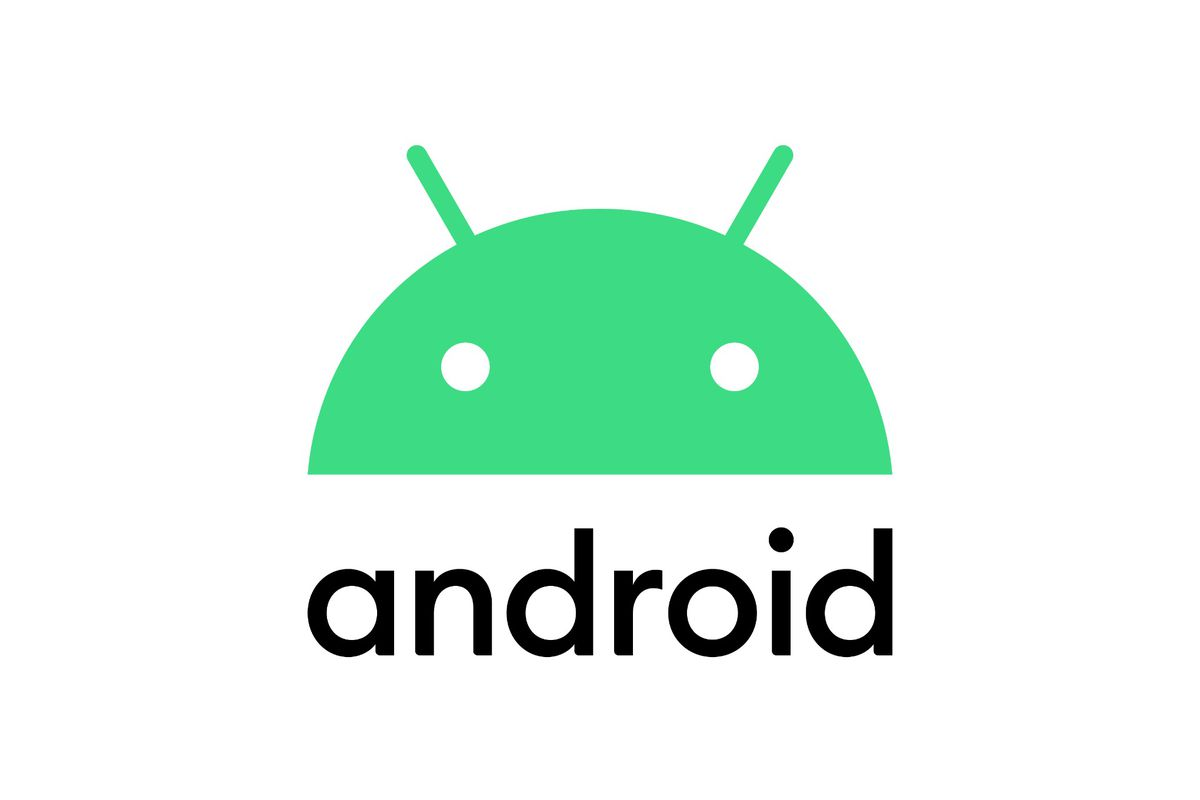
\includegraphics[scale=0.2]{pictures/logo_android.jpg}
    \caption{Logo Android}
\end{figure}

Android adalah sistem operasi dengan basis linux yang dirancang untuk perangkat yang bergerak atau layar sentuh \textit{touchscreen} seperti telepon pintar \textit{smartphone} dan \textit{tablet}. Android merupakan sistem operasi \textit{open source} (aplikasi yang tidak dipegang hanya untuk seorang saja tetapi orang lain bisa menggunakan \textit{sourcecode} tersebut). Android ini mengunakan lisensi dari Google yang kodenya tersebut berada dibawah Lisensi \textit{Apache}. Lisensi \textit{Apache} merupakan lisensi yang bebas untuk \textit{software} yang ditulis oleh \textit{Apache Software Foundation} (ASF).

Android berdiri pada bulan Oktober 1980, tepatnya di Palo Alto,  California. Android ini didirikan oleh Andy Rubin, Rich Muner, Nick Sears, dan Chris White. Android dikembangkan oleh perusahaan dengan nama \textit{Ancroid.inc}. Pada tahun 2005 perusahaan tersebut mendapatkan dukungan finansial dari \textit{google.inc}

Pada awalnya Android tidak dibbuat untuk ponsel, namun android pertama kali dibuat untuk kamera digital. Tetapi, dengan melihat peluang yang lebih besar jika Android digunakan untuk perangkat \textit{mobile}, maka Android digunakan pada perangkat \textit{mobile} yang ditujukan untuk menyaingi \textit{Symbian} dan \textit{Windows Mobile}.

Secara resmi, Android dirilis pada tahun 2007 bersamaan dengan berdirinya \textit{Open Handset Alliance}. \textit{Open Handset Alliance} merupakan \textit{Open Source Developer} bagi perangkat \textit{mobile} atau seluler. Tahun 2008, \textit{Handphone} pertama yang menggunakan sistem operasi android kemudian dirilis, \textit{handphone} ini bernama \textit{HTC Dream}. Dua tahun setelah perilisan \textit{Handphone} ini, Google menyusul dengan merilis \textit{Smartphone} dengan seri \textit{Nexus One} yang proses pembuatannya dibantu oleh \textit{HTC}. Dengan dirilisnya \textit{Handphone} tersebut, memancing kemunculan-kemunculan berbagai brand dari \textit{OEM} yang bermacam-macam. Dimulai dari \textit{Samsung, Lenovo, HTC, ASUS, LG} dan masih banyak lagi.

\begin{figure}[!htbp]
    \centering
    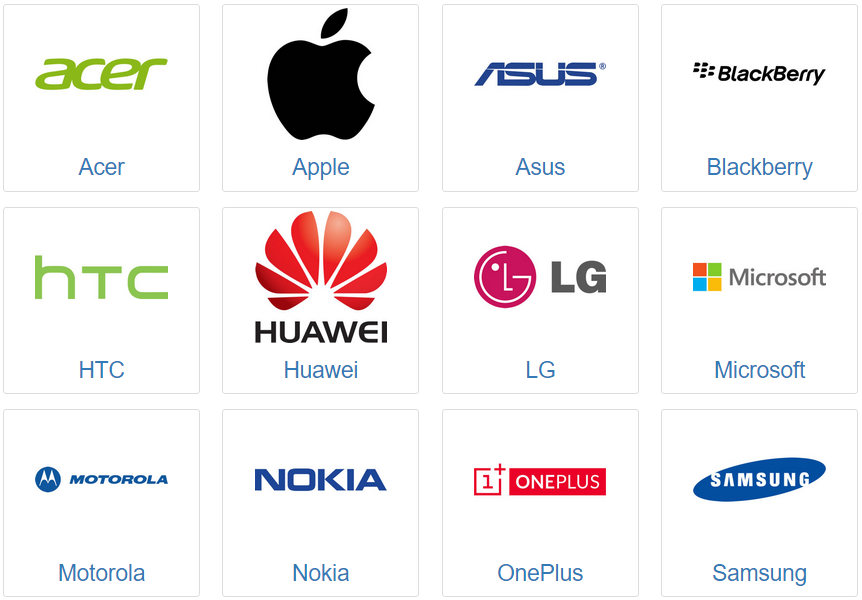
\includegraphics[scale = 0.3]{pictures/merk-OEM-Android.png}
    \caption{OEM Android Smartphone}
\end{figure}

Selain berfokus pada \textit{smartphone}, Google juga banyak mengembangkan aplikasi Android untuk perangkay lainnya. Contohnya Google mengembangkan Android TV yang digunakan untuk televisi, Android Auto yang digunakan pada, dan Android Wear pada jam tangan. Aplikasi android tersebut memiliki \textit{Interface} yang berbeda beda sesuai dengan kebutuhan dan fungsionalitasnya masing-masing. 

\textit{Open Source Code} dan lisensi yang diguakan pada Android tentunya dapat membuat Sistem Operasi ini dapat diubah-ubah dan dimodifikasi dengan bebas yang kemudian dapat di distribusikan oleh para \textit{developer} Android itu sendiri. Selain mudah untuk digunakan, Android memiliki \textit{Developer Community} (Komunitas Pengembang) sendiri yang dapat memperluas fungsionalitas dari perangkat yang umumnya digunakan menggunakan bahasa pemrograman \textit{Java}. Selain \textit{java}, Android ini juga dapat menggunakan bahasa pemrograman \textit{Kotlin}. Lebih dari Satu juta aplikasi kemudian tersedia untuk android, dan miliaran aplikasi telah melakukan di\textit{download} dari \textit{Google Play} (toko utama yang berisi aplikasi-aplikasi dari Android)

Dimulai sejak tahun 2008, Android melakukan pembaruan untuk meningkatkan kinerja aplikasinya secara bertahap dengan cara menambahkan fitur-fitur yang baru dan memperbaiki \textit{error} dan \textit{bug} yang terdapat pada produk dengan versi yang sebelumnya. Setiap versi dari android biasanya disusun dengan nama alfabetis dan nama yang digunakan adalah nama makanan-makanan yang ringan atau cemilan. Sebagai contoh pada android versi 7.0 yang diberi nama Android \textit{Nougat}, Kemudian Android 8.0 yang diberi nama \textit{Oreo} dan seterusnya. 

\section{Versi Pada Android}
Pada awal kemunculan Android, Android telah mengeluarkan banyak versi. Setiap versi dari android ini tentunya memiliki fitur-fiturnya masing-masing sesuai dengan perkembangan zaman. Hal ini tentunya sebagai cara agar mengalahkan pesaingnya yang menggunakan OS yang lainnya seperti Apple iOS, Windows, Blackberry, Symbian dan lainnya. 
\begin{enumerate}

\item Android 1.0 \textbf{Apple Pie}\\
\begin{figure}[!htbp]
    \centering
    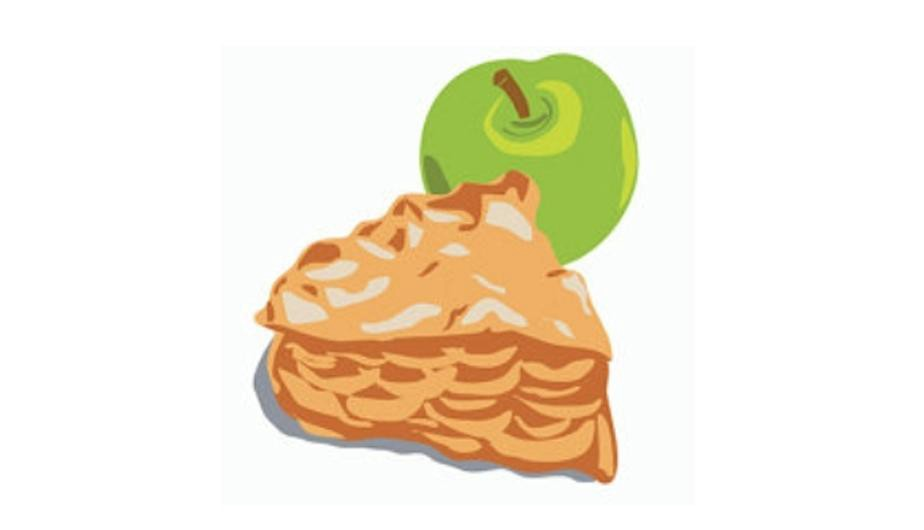
\includegraphics[scale = 0.3]{pictures/android-apple-pie.jpg}
    \caption{Android Apple Pie}
    \label{}
\end{figure}

Android versi pertama ini merupakan android dengan versi 1.0 yang diberi nama Android \textit{Apple Pie} yang dirilis oleh android  pada 23 September 2008 dan hanya memiliki fitur yang terbatas. Fitur fitur tersebut adalah:

\begin{enumerate}
    \item \textit{Play Store}
    \item Kamera
    \item \textit{Web Browser}
    \item \textit{G-Mail Sychronization}
    \item Kontak
    \item Google Agenda
    \item Google \textit{Maps}
\end{enumerate}
Selain itu, Android versi ini juga sudah mendukung fasilitas youtube. Setidaknya Google dan OHA telas merilis 2 versi saat sebelum Android beta yang dirilis pada bulan November 2007. Pada Android Versi Alpha memiliki sebutan atau \textit{codename} \textit{Astro Boy, Bender,} dan R2-D2.\\

KELEBIHAN
\begin{enumerate}

\item Android Market\\ 
Android market merupakan aplikasi untuk \textit{mendownload} dan \textit{mengupdate} aplikasi yang terinstall melalui toko resmi dari Android.
\item \textit{Web Browser}\\
Android \textit{Web Browser} merupakan aplikasi untuk \textit{searching website}, menampilkan halaman \textit{Web HTML} dan \textit{XHTML} dan dapat digunakan untuk melihat halaman web dengan \textit{fullscreen} dan dapat juga diperbesar.
untuk menampilkan, memperbesar dan melihat dalam layar penuh halaman \textit{Web HTML} dan \textit{XHTML}
\item Kamera
\item Memungkinkan pengelompokan ikon-ikon aplikasi ke dalam satu folder pada bagian layar utama (\textit{homescreen}).
\item Dapat memiliki dan mengakses \textit{E-Mail}, mendukung fasilitas POP3, IMAP4, dan SMTP
\item Sinkronisasi \textit{G-mail} dengan menggunakan aplikasi \textit{G-mail}.
\item Sinkronisasi \textit{Google Contacts} dengan menggunakan aplikasi \textit{People}.
\item Sinkronisasi \textit{Google Calendar} dengan menggunakan aplikasi \textit{Calendar}.
\item Aplikasi \textit{Google Maps} \\
Aplikasi \textit{Google Maps} ini menyediakan informasi mengenai Latitude, derdapat fitur \textit{Street View}, dapat melihat melihat peta dan tampilan melalui citra satelit, menemukan lokasi yang akan dituju dan dapat memberi petunjuk arah saat mengemudi kendaraan maupun saat berjalan-jalan.
\item \textit{Google Sync}\\ 
Fitur ini dapat memungkinkan pengelolaan sinkronisasi pada aplikasi \textit{Gmail, People, dan Calendar}.
\item Google Search\\
Fitur ini dapat memungkinkan pengguna untuk \textit{Searching} sesuatu menggunakan \textit{website}.
\item \textit{Google Talk} \\
\textit{Google Talk} merupakan sebuah aplikasi pesan instan yang diproduksi oleh google
\item Pesan instan, pesan teks (SMS), dan MMS.
\item \textit{Media Player}\\
\textit{Media Player}ini digunakan untuk mengelola, mengimpor, dan memutar file yang mendukung pada berkas penyimpanan. Tetapi, pada versi ini belum menyediakan dukungan \textit{Video} dan \textit{Bluetooth Stereo}
\item Notifikasi\\
Notifikasi ini merupakan fitur yang akan muncul pada status bar, dengan diberikan pilihan pengaturan untuk mengatur \textit{Ringtone}, cahaya \textit{LED} yang dikeluarkan maupun nada getar.
\item \textit{Voice Dialer}\\ 
\textit{Voice Dialer} ini memberikan akses kepada pengguna untuk memanggil kontak tanpa harus mengetikan nama ataupun nomor telepon orang yang akan dituju.
\item Wallpaper\\ 
Fitur ini dapat digunakan pengguna untuk mengatur gambar \textit{Wallpaper} pada \textit{Homescreen} perangkat android pengguna. 
\item \textit{Youtube Video Player}
\item Fitur Pendukung Lainnya seperti:
\begin{enumerate}
    \item Jam Alarm
    \item Kalkulator
    \item Panggilan
    \item \textit{Homescreen Launcher}
    \item Galeri
    \item Pengaturan
\end{enumerate}
\item Wi-Fi
\item Bluetooth\\
\end{enumerate}

KEKURANGAN
\begin{enumerate}
    \item Versi Android ini pada awalnya belum memiliki nama yang cocok sehingga tidak diberi nama dan hal tersebut dapat membuat bingung masyarakat karena tidak akan mudah untuk diingat.\\
\end{enumerate}


\item Android 1.1 \textbf{Banana Bread}\\
\begin{figure}[!htbp]
    \centering
    
\includegraphics[scale = 1.2]{pictures/android-banana-bread.jpg}
    \caption{Android Banana Bread}
    \label{}
\end{figure}

Pada Februari 2009, Android meng-\textit{upgrade} dari versi sebelumnya (versi 1.0) ke versi 1.1 yang bernama Android \textit{Banana Bread}. Fitur pada android ini tidak jauh bedanya dengan versi sebelumnya. \textit{Smartphone} pertama yang menggunakan versi ini adalah \textit{HTC}. Android 1.1 \textit{Banana Bread} ini memiliki nama lain yaitu \textit{"Petit Four"}. Nama ini tentunya bukan nama resmi yang dikeluarkan oleh pihak Android. Versi ini merupakan versi yang berkembang dan memperbaiki beberapa bug (\textit{Error}) yang ada pada Android sebelumnya. Versi ini juga mengubah \textit{API} dari android yang sebelumnya. Selain itu, Android ini menambahkan fitur fiitur baru yaitu:
\begin{enumerate}
    \item \textit{Maps} dan pencarian lokasi bisnis sudah terdapat rincian tempat.
    \item Tombol Panggilan yang dapat di sembunyikan atau di tampilkan.
    \item Dapat menyimpan lampiran dalam pesan
    \item Mendapat dukungan \textit{Marquee} pada ruang sistem.\\
\end{enumerate}


\item Android 1.5 \textbf{Cupcake}\\
\begin{figure}[!htbp]
    \centering
    
\includegraphics[scale = 0.3]{pictures/android-cupcake.jpg}
    \caption{Android Cupcake}
    \label{}
\end{figure}

Adroid Versi ini diluncurkan pada bulan April 2009 dan tidak memiliki perbedaan yang signifikan dengan versi Android yang terdahulu. Meski dengan sedikit perbedaan, android ini mendapatkan fitur tambahan seperti \textit{Support Bluetooth A2DP, AVRCP, Soft Keyboard} dengan \textit{Text Suggestion, Record} ataupun \textit{Watch Videos}. Android ini merupakan versi Android yang mulai menggunakan nama makanan cemilan yaitu "\textit{Cupcake}". Pada Android versi ini, terdapat pembaruan, penambahan fitur, dan Perubahan \textit{User Interfaces}, beberapa perubahannya yaitu:
\begin{enumerate}
    \item \textit{Third Party Virtual Keyboard} dengan prediksi teks dan \textit{User Dictionary}(Kamus pengguna)
    \item Mendapat dukungan \textit{Widget}
    \item Sudah memiliki kemampuan \textit{record video} dan memutar video dengan format MPRG-4 (.mp4) dan .3gp
    \item Memiliki fasilitas \textit{pairing bluetooth}
    \item Mendukung \textit{bluetooth stereo} \textit{A2DP dan AVRCP}
    \item Penambahan fitur \textit{Copy and Paste} pada \textit{Web Browser}
    \item Fitur Menambahkan foto pada kontak telepon
    \item Pada bagian panggilan, tanggal dan waktu ditampilkan di bagian log panggilan
    \item Dapat memanggil kontak melali log panggilan
    \item Animasi saat terjadi transisi layar
    \item Fitur \textit{Auto Rotate} (Putar Otomatis)
    \item Update Animasi saat \textit{Booting} OS 
    \item Dapat \textit{Upload} video ke youtube
    \item Dapat \textit{Upload} foto ke picasa\\
\end{enumerate}


\item Android 1.6 \textbf{Donut}\\
\begin{figure}[!htbp]
    \centering
    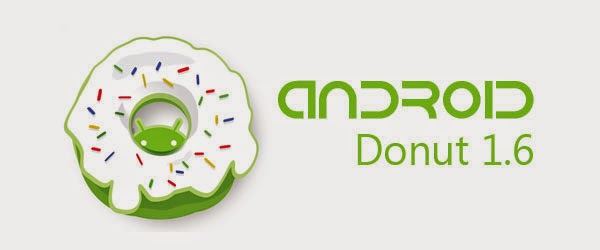
\includegraphics[scale=0.5]{pictures/android_donut.jpg}
    \caption{Android Donut}
    \label{}
\end{figure}

Android Versi 1.6 atau dikenal dengan Android \textit{Donut} merupakan versi android yang dirilis pada tanggal 15 September 2009, dan terdapat fitur-fitur tambahan dari versi yang sebelumnya. Android ini memiliki sedikit kesalahan (bug atau \textit{error}) pada sistemnya. Selain itu, Android ini memiliki fitur yang cukup banyak yang ditambahkan oleh Google sehingga Android ini terbilang Android dengan versi yang cukup sempurna pada zamannya. Fitur-fitur tambahan pada Android versi ini adalah sebagai berikut:
\begin{enumerate}
    \item Terdapat fitur pencarian suara dan teks dalam \textit{history, bookmark,} kontak dan web.
    \item Fitur untuk menyertakan konten pada \textit{Developer} pada hasil pencarian.
    \item \textit{Voice machine} yang dapat mengucapkan berbagai bahasa dan membuat Android tertentu dapat mengucapkan teks.
    \item Pencarian menjadi lebih mudah
    \item Kemampuan untuk melihat sedikit cuplikan aplikasi di \textit{Android Market}
    \item Galeri, Kamera dan \textit{Video recorder} yang terintegrasi
    \item Akses Kamera lebih cepat
    \item Dapat memilih \textit{multifiles} untuk menghapus foto dalam sekala banyak.
    \item \textit{Update} pada teknologi \textit{CDMA/EVDO, 802.1x, VPN} dan mesin pengucap teks
    \item Mendukung resolusi layar \textit{WVGA}
    \item Peningkatan pencarian dan kamera
    \item Memperluas kerangka kerja, Gestur dan penambahan \textit{tools GestureBuilder Developer}.\\
\end{enumerate}

KEKURANGAN
\begin{enumerate}
    \item Hanya aplikasi tertentu yang dapat diinstall disini.
    \item Tidak ada \textit{equalizer} pada \textit{Music Player}nya.
    \item Android market tidak terintegrasi
    \item Keypad yang lambat
    \item \textit{Touch Responsiveness} kurang.\\
\end{enumerate}


\item Android 2.0 \textbf{Eclair}
\begin{figure}[!htbp]
    \centering
    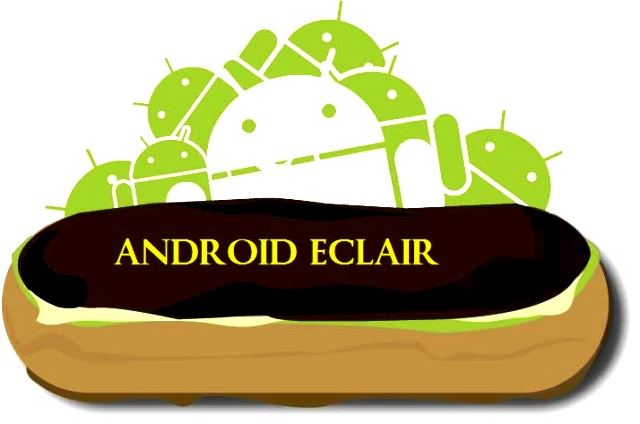
\includegraphics[scale=0.3]{pictures/android-eclair.jpg}
    \caption{Android Eclair}
    \label{}
\end{figure}

Android versi 2.0 ini bernama android \textit{eclair} yang dirilis pada tanggal 26 Oktober 2009. Android versi ini memiliki beberapa jenis \textit{API level} yaitu:
\begin{enumerate}
    \item Android Eclair 2.0 (API level 5)\\
    Android versi 2.0 ini dirilis pada tanggal 26 Oktober 2009. Pada Android versi ini memiliki beberapa fitur tambahan dari versi-versi sebelumnya. Perubahan fitur pada android versi ini adalah:
    \begin{enumerate}
        \item Bluetooth 2.1
        \item \textit{Multi-touch system}
        \item \textit{Live wallpaper}
        \item \textit{Flash} kamera, \textit{Digital Zoom, Skin mode, macro focus}
        \item HTML
        \item \textit{Digital Zoom}
        \item \textit{Support Microsoft Exchange}
        \item Update pada UI \textit{Web Browser} dengan fitur \textit{bookmark, double tap zoom, support HTML5}
        \item Multi akun pada saat sinkronisasi menggunakan \textit{E-Mail} dan kontak
        \item \textit{E-Mail} untuk \textit{Microsoft Exchange} dengan kemampuan untuk mencari \textit{E-Mail} dari beberapa akun dalam satu halaman
        \item Dapat memilih foto kontak
        \item Opsi untuk memanggil, mengirim sms dan \textit{E-Mail} pada kontak 
        \item Mampu mencari SMS dan MMS yang tersumpan. Pesan yang terlalu lama akan terhapus dengan sendirinya jika sudah mencapai batas maksimum.
        \item Kecepatan \textit{keyboard virtual} lebih cepat dan \textit{support} kamus yang mempelajari kata dan nama kontak
        \item Menyempurnakan UI dari kalender, menampilkan notifikasi kalender.
        \item Kecepatan \textit{Software} lebih optimal
        \item Resolusi layar lebih beragam
        \item \textit{Update google maps} ke versi 3.1.2
    \end{enumerate}
    
    \item Android Eclair 2.0.1 (API level 6)\\
    Android ini dirilis pada tanggal 3 Desember 2009. Versi ini merupakan \textit{update} dari versi sebelumnya (Android Eclair 2.0). \textit{Update} yang terdapat pada versi ini adalah:
    \begin{enumerate}
        \item Perubahan minor pada API nya
        \item Perbaikan pada bug yang terjadi di versi sebelumnya
        \item Perubahan \textit{workflow}(Kerangka kerja) pada sistemnya
    \end{enumerate}

    \item Android Eclair 2.1 (API level 7)\\
    Android ini dirilis pada tanggal 12 Januari 2010. Versi ini merupakan \textit{update} dari versi sebelumnya (Android Eclair 2.0.1). \textit{Update} yang terdapat pada versi ini adalah:
    \begin{enumerate}
        \item Perubahan Minor pada API nya
        \item Perbaikan pada bug yang terjadi di versi sebelumnya\\
    \end{enumerate}
\end{enumerate}

\item Android 2.2.9 \textbf{Froyo}\\
\begin{figure}[!htbp]
    \centering
    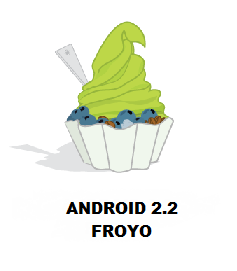
\includegraphics[scale = 0.45]{pictures/android-froyo.png}
    \caption{Android Froyo}
    \label{}
\end{figure}

Android 2.2.9 atau dikenal dengan nama android Froyo, diluncurkan pada Mei 2010. Versi ini dirilis oleh perusahaan besar yaitu Google. Versi ini merupakan versi penyempurna dari versi versi yang sebelumnya. Versi ini dibentuk dengan tujuan untuk meningkatkan kinerja dari sistem Android. Fitur fitur yang terdapat pada versi android ini adalah: 
\begin{enumerate}
    \item Peningkatan kecepatan sistem
    \item Pengimplementasian JIT
    \item Integrasi mesin dari JavaScript V8 Chrome kedalam \textit{Web Browser}
    \item Dukungan \textit{Android Cloud to Device Messaging (C2DM) }
    \item Meningkatkan \textit{Microsoft Exchange Support}, keamanan, pencarian otomatis, GAL, sinkronisasi pada kalender dan pembersihan dari jarak jauh
    \item Memberikan fitur \textit{Shortcut} untuk launcher terutama \textit{shortcut} pada telepon dan \textit{web browser}.
    \item USB Tethering
    \item Fitur untuk mengaktifkan dan menonaktifkan paket data jaringan seluler
    \item Menambahkan otomatis \textit{update} pada aplikasi \textit{Market}
    \item dapat membagikan kontak dan panggilan suara melalui bluetooth
    \item Mendapat dukungan \textit{Bluetooth enable car} dan  \textit{desk docks}
    \item Mendukung \textit{Password alphanumeric}
    \item Aplikasi untuk mengontrol \textit{space} pada memori atau storage
    \item Mendukung upload file melalui \textit{web browser}
    \item Mendukung animasi GIF
    \item Mendapat dukungan \textit{Adobe Flash}
    \item Mendukung tampilan PPI (maksimal hingga 320 ppi), misalnya layar 4 inch dengan resolusi 720p
    \item \textit{Zoom} pada galeri
\end{enumerate}

\item Android 2.3 \textbf{Gingerbread}\\
\begin{figure}[!htbp]
    \centering
    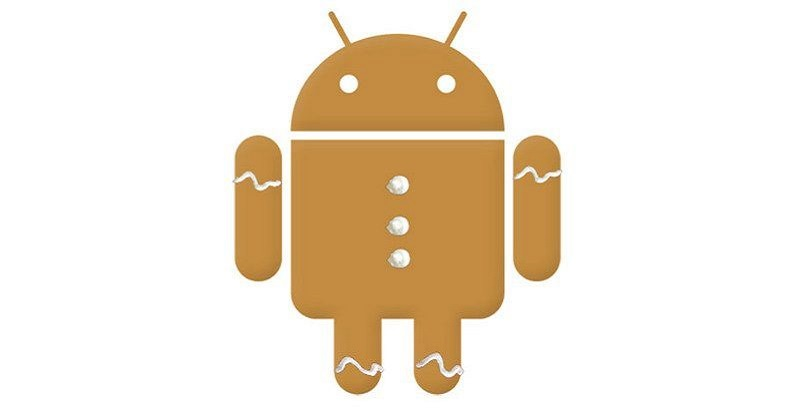
\includegraphics[scale = 0.3]{pictures/android-gingerbread.jpg}
    \caption{Android Gingerbread}
    \label{}
\end{figure}

Android 2.3 atau biasa disebut Android \textit{Gingerbread} merupakan versi android yang dikeluarkan pada bulan Desember 2010. Secara fitur, Android ini sudah tergolong sempurna dan ditambah lagi pada android 2.3 ini telah diadopsi oleh sebuah perusahaan yang membuat \textit{Smartphone} yang sangat terkenal dan terpopuler dengan merek Samsung dengan menanamkan OS ini ke dalam \textit{Smartphonenya}. Smartphone yang digunakan adalah smartphone seri \textit{Nexus} dengan menggunakan fitur-fitur seperti:
\begin{enumerate} 
    \item Memperbarui desain UI nya dengan mempercepat kerja UI dan menyederhanakannya.
    \item Resolusi dan layar dibuat menjadi besar (WXGA dan tingkat yang lebih tinggi)
    \item Dukungan telepon internet SIP VoIP
    \item Input untuk teks yang lebih cepat dan lebih intuitif pada \textit{Keyboardnya} Cara tersebut ditingkatkan dengan meninggkatkan akurasi, \textit{Text Suggestion} dan  \textit{input} dengan menggunakan suara
    \item \textit{Upgrade} fungsi \textit{Copy and Paste} yang memungkinkan pengguna untuk memilih kata dengan menekan layar. 
    \item Dukungan untuk NEar Field Communication (NFC), memungkinkan pengguna untuk membaca NFC yang ada pada poster, stiker dan juga iklan. 
    \item Dukungan bagi Near Field Communication (NFC), memungkinkan pengguna untuk membaca tag NFC yang tertanam dalam poster, stiker, atau iklan
    \item Efek audio baru seperti reverb, equalizer, virtualisasi penyuara kuping, dan bass boost
    \item Download Manager baru, memudahkan pengguna untuk mengakses berkas yang diunduh dari penjelajah web, surel, ataupun dari aplikasi lainnya
    \item Dukungan multi kamera pada perangkat, termasuk kamera depan, jika tersedia
    \item Dukungan bagi pemutar video WebM/VP8, dan audio AAC
    \item Peningkatan manajemen daya dengan peran lebih aktif dalam mengelola aplikasi yang beroperasi terlalu lama
    \item Peningkatan dukungan bagi pengembangan kode asli
    \item Peralihan dari YAFFS ke ext4 pada perangkat yang lebih baru
    \item Peningkatan kualitas audio, grafis, dan masukan bagi pengembang permainan
    \item Dukungan sensor yang lebih banyak (seperti giroskop dan barometer)
\end{enumerate}

\item Android 3.0 - 3.2 6 \textbf{Honeycomb}\\
\begin{figure}[!htbp]
    \centering
    
\includegraphics[scale=0.1]{pictures/android-honeycomb.png}
    \caption{Android Honeycomb}
    \label{}
\end{figure}

Honeycomb adalah salah satu sistem operasi Android versi terbaru yang dirilis pada bulan Februari 2011 silam. Namun, versi ini lebih ditujukkan untuk perangkat Tablet yang mana pada tahun itu sangat laris atau laku dipasaran. Beberapa fitur dan perbaikan pada Android Honeycomb, yaitu :
\begin{enumerate}
    \item Support Multi core
    \item Support Tablet lebih baik
    \item Updated 3D UI
    \item Layar Utama (homescreens) yang dapat diatur
    \item Melihat aplikasi yang barusan dibuka
    \item Menyempurnakan layout keyboard
    \item Transport protocol untuk Media atau Picture video chat Google Talk
    \item Google eBooks
    \item “Private browsing”
    \item System-wide Clipboard
    \item HTTP Live streaming
\end{enumerate}
Update 3.1:
\begin{enumerate}
    \item Peningkatan UI
    \item Open Accessory API
    \item USB host API
    \item Support mouse, joysticks dan gamepad
    \item Widget Home screen yang bisa di atur size atau ukurannya
    \item Notificasi MTP
    \item RTP API untuk audio
\end{enumerate}
Update 3.2:
\begin{enumerate}
    \item Optimise pada berbagai tablets
    \item Mode kompatibilitas display (zoom for fixed sized apps)
    \item Sinkronisasi Media dari SD card
\end{enumerate}
Update 3.2.1:
\begin{enumerate}
    \item Update Android Market merupakan automatic updates yang lebih mudah
    \item Update Google Books
    \item Peningkatan kinerja Wi-Fi
    \item Perbaikan prediksi tulisan tangan dengan huruf Chinese
\end{enumerate}
Update 3.2.2:
\begin{enumerate}
    \item Perbaikan kecil
\end{enumerate}
Update 3.2.4:
\begin{enumerate}
    \item Update tambahan ‘Pay as you go’ bagi tablet
\end{enumerate}
Update 3.2.6
\begin{enumerate}
    \item Perbaikan kecil 
\end{enumerate}

\item Android 4.0 \textbf{Ice Cream Sandwich}\\
\begin{figure}[!htbp]
    \centering
    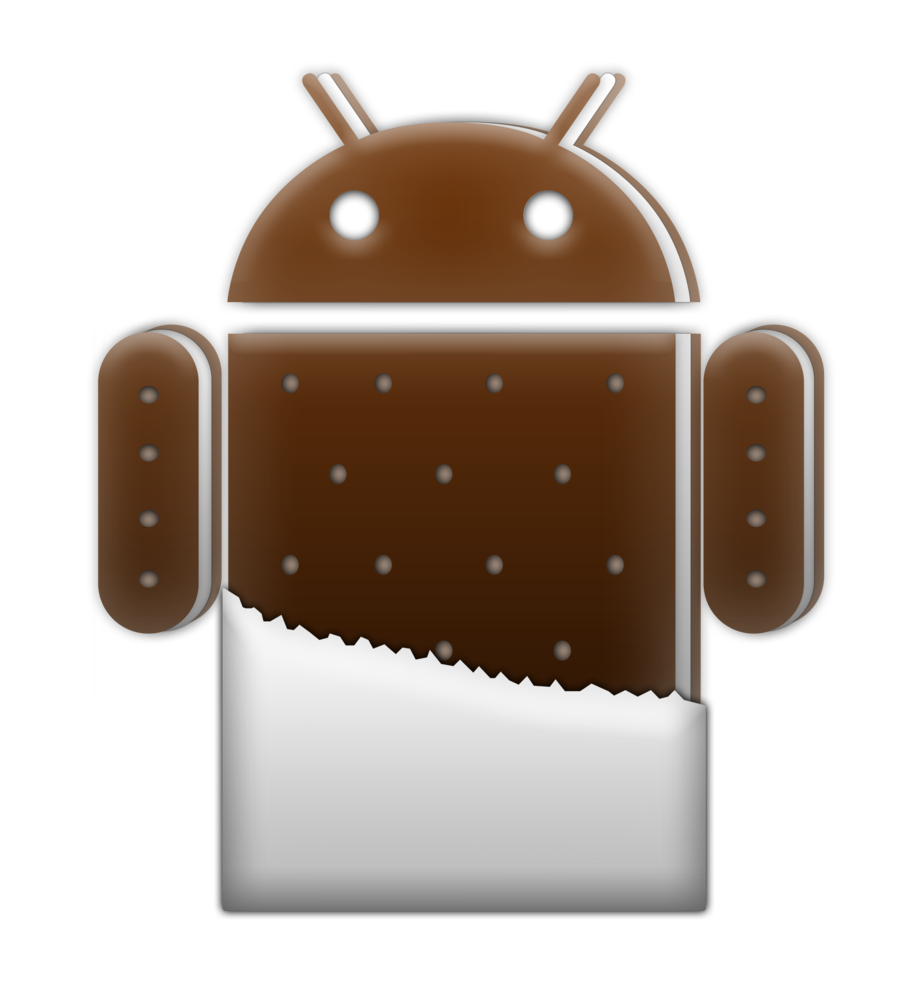
\includegraphics[scale = 0.1]{pictures/android-ice-cream-sandwich.png}
    \caption{Android Ice Cream Sandwich}
    \label{}
\end{figure}

Puncak kesempurnaan Android yakni ketika pada versi ini, dimana Ice Cream Sandwich dirilis pada bulan Oktober 2011 silam. Dan operasi sistem ini mulai bekerja dengan baik di semua jenis smartphone apapun. Selain bertambahnya berbagai fitur yang menarik, Ice Cream Sandwich juga merupakan versi yang paling banyak disukai pada saat itu. Bahkan, Android Ice Cream Sandwich juga sudah dilengkapi dengan fitur ekstra multitasking serta notifikasi yang lebih banyak. Pembaruan pada versi ini antara lain:
\begin{enumerate}
    \item Tombol lunak tablet Android 3.x tersedia bagi penggunaan di telepon pintar
    \item Pemisahan widget di tab baru, terletak pada layar yang bersebelahan dengan aplikasi
    \item Pembuatan folder yang lebih mudah, dengan gaya drag-and-drop
    \item Launcher yang bisa dikustomisasi
    \item Peningkatan fitur pesan suara visual, dengan kemampuan untuk mempercepat atau memperlambat kecepatan pesan suara
    \item Fungsi ‘cubit untuk memperbesar’ pada kalender
    \item Pengintegrasian fungsi cuplikan layar (screenshot) dengan menekan dan menahan tombol daya dan volume-turun secara bersamaan
    \item Perbaikan kesalahan koreksi pada papan ketik
    \item Kemampuan untuk mengakses aplikasi secara langsung dari layar kunci (lock screen)
    \item Perbaikan fungsi salin dan tempel
    \item Integrasi suara yang lebih baik dan berkesinambungan
    \item Mode buka kunci identifikasi wajah, fitur yang memungkinkan pengguna untuk membuka perangkat menggunakan perangkat lunak pengenal wajah
    \item Penambahan penjelajah web bawaan Chrome, mampu membuka halaman hingga 16 tab
    \item Sinkronisasi otomatis pada penjelajah web dengan bookmark Chrome pengguna
    \item Penambahan jenis huruf baru, Roboto
    \item Penggunaan data bisa dibatasi, pengguna akan diperingatkan jika penggunaan data sudah mendekati batas tertentu, dan menonaktifkan data yang digunakan ketika batas tersebut terlampaui
    \item Kemampuan untuk mematikan aplikasi yang menggunakan data di latar belakang
    \item Peningkatan fungsi aplikasi kamera dengan fitur-fitur seperti zero shutter lag, time lapse settings, mode panorama, dan kemampuan untuk memperbesar saat merekam video
    \item Penambahan aplikasi pengedit foto bawaan
    \item Tata letak galeri yang baru, bisa dikelola berdasarkan lokasi dan orang
    \item Pemutakhiran aplikasi “People” dengan integrasi pada jejaring sosial
    \item Android Beam, fitur komunikasi area dekat yang memungkinkan dilakukannya pertukaran jarak pendek bookmark web, info kontak, arah, video YouTube, dan data lainnya
    \item Dukungan format gambar WebP
    \item Merekam video 1080p bagi perangkat Android tertentu
    \item Modul kernel Android VPN Framework (AVF) dan TUN (bukan TAP). Sebelum versi 4.0, perangkat lunak VPN membutuhkan rooting.
\end{enumerate}

\item Android 4.1.2 \textbf{Jelly Bean}
\begin{figure}[!htbp]
    \centering
    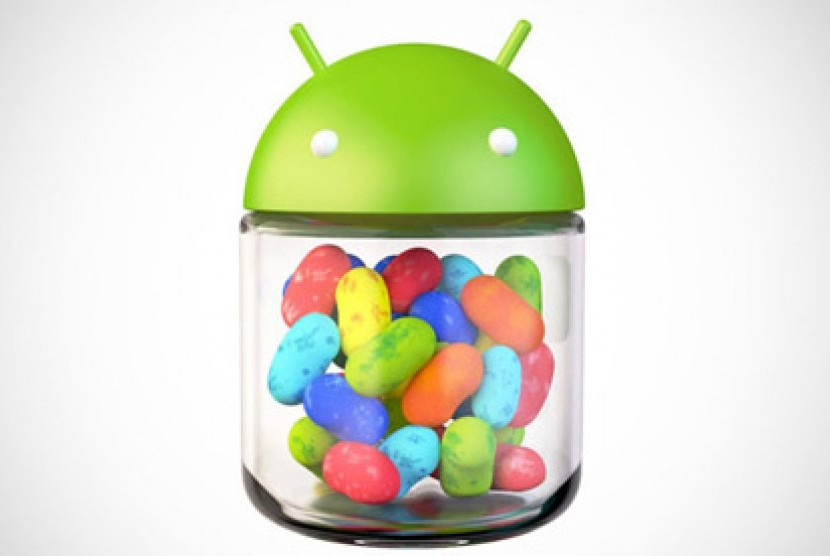
\includegraphics[scale=0.25]{pictures/android-jelly-bean.jpg}
    \caption{Android Jelly Bean}
    \label{}
\end{figure}

Jelly Bean dirilis pada 9 Juli 2012 lewat konferensi I/O Google. Versi ini adalah salah satu versi Android yang kerap mendapatkan update fitur-fitur yang bermanfaat dan menarik, beberapa contohnya semacam memperbaiki rotasi layar, seperti Support resolusi video 4K, Support penulisan huruf Hebrew dan Arabic dari kanan ke kiri, peningkatan kinerja, dan sistem keamanan serta masih banyak lainnya. Fitur yang terdapat pada versi ini adalah : 
\begin{enumerate}
    \item Antarmuka pengguna yang lebih halus:
    \item Waktu vsync pada animasi UI dikelola oleh kerangka kerja Android, termasuk reaksi aplikasi, efek sentuh, komposisi layar, dan penyegaran tampilan
    \item Triple buffering pada grafis
    \item Peningkatan aksesbilitas
    \item Teks dua bahasa dan dukungan bahasa lainnya
    \item Papan ketik yang bisa dimodifikasi oleh pengguna
    \item Perluasan notifikasi
    \item Kemampuan untuk mematikan notifikasi pada aplikasi tertentu
    \item Shortcut dan widget secara otomatis bisa disusun ulang atau diatur ukurannya
    \item Transfer data Bluetooth bagi Android Beam
    \item Diktasi suara luring
    \item Tablet dengan layar kecil bisa menyesuaikan tata letak antarmuka dan layar depan seperti pada telepon pintar
    \item Peningkatan pencarian suara
    \item Peningkatan aplikasi kamera
    \item Google Wallet (pada Nexus 7)
    \item Foto kontak Google+ resolusi tinggi
    \item Aplikasi pencarian Google Now
    \item Audio multi-saluran
    \item Audio USB (bagi suara eksternal DACs)
    \item Audio chaining
    \item Penjelajah web bawaan Android diganti dengan Google Chrome pada perangkat Android pra-instal
    \item Kemampuan untuk menambahkan widget aplikasi tanpa akses root
\end{enumerate}

\item Android 4.4 \textbf{Kitkat}\\
\begin{figure}[!htbp]
    \centering
    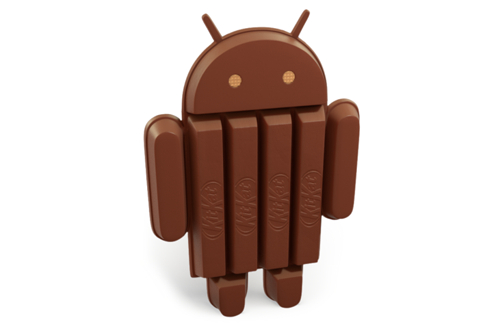
\includegraphics[scale=0.3]{pictures/android-kitkat.jpg}
    \caption{Android Kitkat}
    \label{}
\end{figure}

Android versi inilah yang saat ini banyak dipakai oleh mayoritas masyarakat Indonesia. Kitkat dirilis pada tahun 2013 lalu. pada versi ini, Android banyak mendapatkan pembaharuan/update fitur. Seperti, terdapatnya fitur Screen recording, untuk merekam kegiatan yang terjadi pada layar smartphone, Peningkatan akses notifikasi, New Translucent system UI, System wide settings untuk closed captioning, dan Peningkatan kinerja serta lain sebagainya. Fitur yang terdapat pada versi ini adalah : 
\begin{enumerate}
    \item Pembaruan antarmuka dengan bar status dan navigasi transparan pada layar depan.
    \item Optimasi kinerja pada perangkat dengan spesifikasi yang lebih rendah
    \item Kerangka kerja pencetakan
    \item NFC Host Card Emulation sebagai emulator kartu pintar
    \item WebViews berbasis Chromium
    \item Perluasan fungsionalitas bagi layanan pendengar notifikasi
    \item API umum untuk mengembangkan dan mengelola klien pesan teks, kemampuan untuk menentukan aplikasi SMS standar.
    \item Kerangka kerja baru untuk transisi UI
    \item Kerangka kerja akses penyimpanan untuk mengambil konten dan dokumen dari sumber lain
    \item Sensor batching, Step Detector, dan Counter API
    \item Peningkatan tampilan mode layar penuh, tombol perangkat lunak dan status bar bisa diakses dari tepi dengan cara menggesek
    \item Penyeimbang audio, pemantauan audio, dan peningkatan suara audio
    \item Perekam aktivitas layar yang terintegrasi
    \item Inframerah
    \item Peningkatan aksesibilitas API
    \item Mesin virtual eksperimental baru, ART
    \item Dukungan Bluetooth Message Access Profile (MAP)
\end{enumerate}

\item Android 5.0 \textbf{Lollipop}\\
\begin{figure}[!htbp]
    \centering
    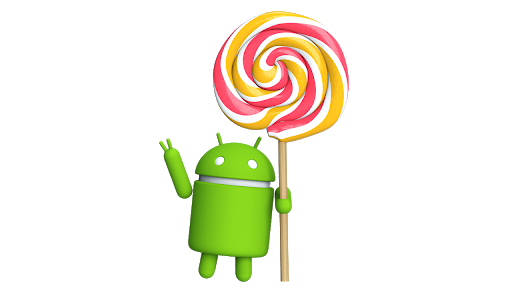
\includegraphics[scale =0.5]{pictures/android-lolipop.png}
    \caption{Android Lollipop}
    \label{}
\end{figure}

Dirilis pada tahun 2014, Android Lollipop lebih banyak menawarkan fitur tambahan untuk menyempurnakan berbagai fitur yang sudah ada. Dan Nexus 6 merupakan salah satu ponsel yang pertama mencicipi Android Lollipon ini. Selain itu, Google juga lebih menyempurnakan pada kinerja dari Android Lollipop sendiri. Fitur yang terdapat pada versi ini adalah : 
\begin{enumerate}
    \item Desain antarmuka (tampilan) yang dinamakan “Material Design”.
    \item 64-bit ART compiler
    \item Project volta, yang berguna untuk meningkatkan daya hidup baterai 30 persen lebih tahan lama.
    \item ‘factory reset protection’. Fitur ini berguna ketika smartphone hilang, ia tidak bisa direset ulang tanpa memasukkan id google dan kata sandi (password).
\end{enumerate}

\item Android 6.0 \textbf{Marshmallow}\\
\begin{figure}[!htbp]
    \centering
    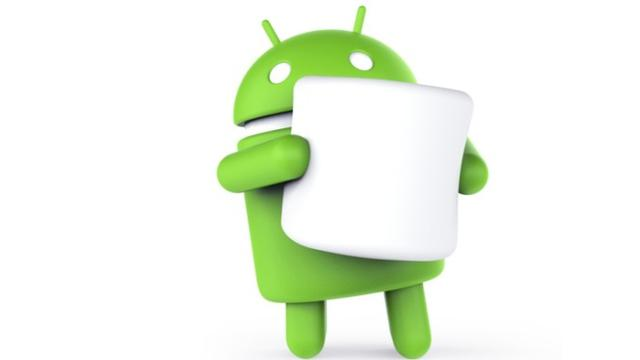
\includegraphics[scale=0.3]{pictures/android-marshmallow.jpg}
    \caption{Android Marshmallow}
    \label{}
\end{figure}

Android versi 6.0 dirilis pada tahun 2015 silam, yang banyak membawa pembaharuan. Salah satunya yaitu suda support USB Type-C. Selain itu, Android Marshmallow ini juga terdapat fasilitas autentikasi sidik jari dan daya baterai yang lebih baik. 

Android Marshmallow memperkenalkan model izin yang didesain ulang: sekarang ada hanya delapan kategori izin, dan aplikasi yang tidak lagi secara otomatis diberikan semua hak akses mereka ditentukan pada waktu instalasi. Sebuah sistem opt-in sekarang digunakan, di mana pengguna akan diminta untuk memberikan atau menolak izin individu (seperti kemampuan untuk mengakses kamera atau mikrofon) untuk aplikasi ketika mereka dibutuhkan. Aplikasi mengingat hibah izin mereka, dan mereka dapat disesuaikan oleh pengguna setiap saat. Model izin baru akan digunakan hanya oleh aplikasi yang dikompilasi untuk Marshmallow menggunakan kit pengembangan perangkat lunak (SDK) tersebut, sementara semua aplikasi lainnya akan terus menggunakan model izin sebelumnya.\\

Marshmallow juga memiliki skema manajemen daya baru bernama Doze yang mengurangi tingkat aktivitas aplikasi latar belakang saat perangkat menentukan bahwa itu tidak sedang aktif ditangani oleh pengguna, yang, menurut Google, menggandakan pemakaian baterai perangkat. Hal ini juga memperkenalkan pilihan untuk mengatur ulang semua pengaturan jaringan, tersedia untuk pertama kalinya pada Android, yang membersihkan pengaturan terkait jaringan untuk WI-FI, Bluetooth dan koneksi seluler.

Android Marshmallow memberikan dukungan asli untuk pengenalan sidik jari, memungkinkan penggunaan sidik jari untuk membuka perangkat dan otentikasi Play Store dan pembelian Android Pay; API standar juga tersedia untuk melaksanakan otentikasi berbasis sidik jari dalam aplikasi lain. Android Marshmallow mendukung USB Type-C, termasuk kemampuan untuk menginstruksikan perangkat untuk mengisi daya perangkat lain melalui USB. Marshmallow juga memperkenalkan “pranala yang diverifikasi” yang dapat dikonfigurasi untuk membuka langsung dalam aplikasi tertentu mereka tanpa petunjuk pengguna lanjut.

Versi API Android yang disediakan oleh Marshmallow adalah 23. Alat pengembang Android Marshmallow tersedia di Pengelola SDK di bawah tingkat API “MNC”.

\item Android 7.0 \textbf{Nougat}\\
\begin{figure}[!htbp]
    \centering
    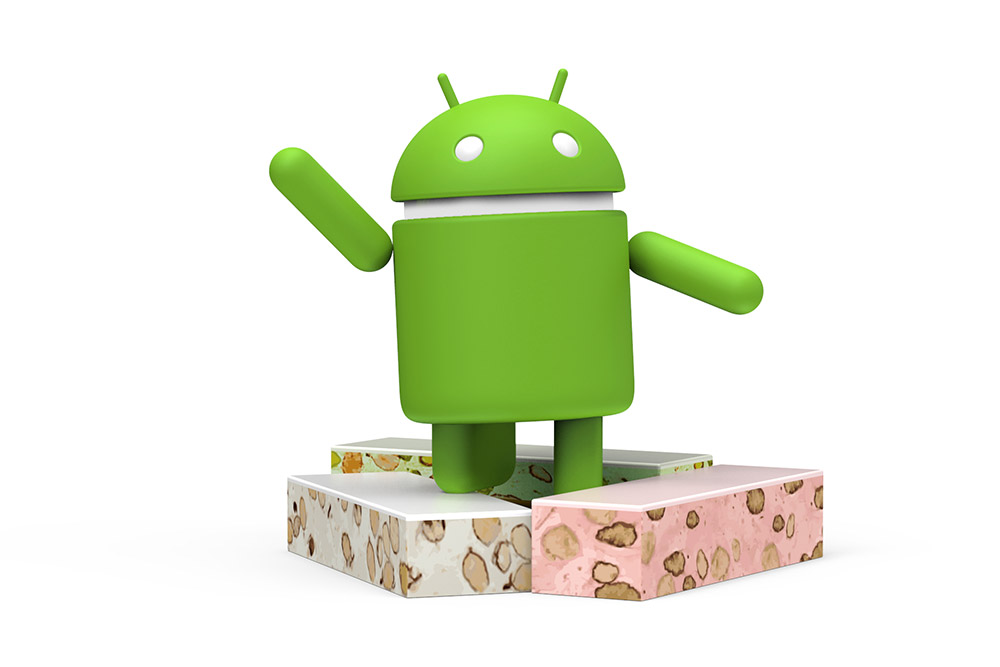
\includegraphics[scale=0.3]{pictures/android-nougat.jpg}
    \caption{Android Nougat}
    \label{}
\end{figure}

Android Nougat versi 7.0 dirilis pada bulan Agustus 2016 yang lebih meningkatkan pada kinerja versi sebelumnya. Selain itu, Android Nougat juga menambah banyak fitur-fitur baru yang diantaranya seperti sudah dapat multitasking, meningkatkan fitur Doze yang dahulu telah dirilis di versi sebelumnya. Inilah beberapa fitur terbaru yang terdapat pada versi Nougat :
\begin{enumerate}
    \item Support Multi window
    \item Dapat langsung membalas pesan dari menu notifikasi atau jendela.
    \item Tampilan panel notifikasi serta quick settings yang baru.
    \item Mode Doze yang lebih baik, (Doze Mode 2.0)
    \item Menu di antara system settings.
\end{enumerate}

\item Android 8.0 \textbf{Oreo}
\begin{figure}[!htbp]
    \centering
    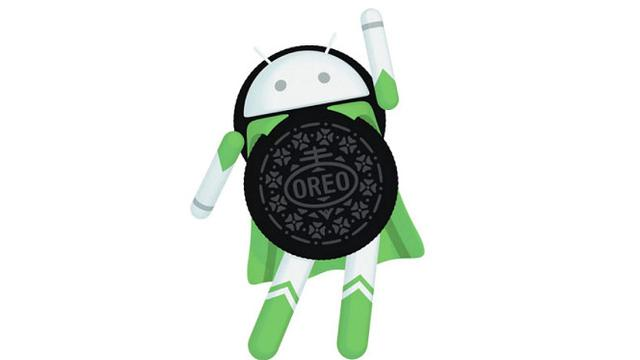
\includegraphics[scale=0.3]{pictures/android-oreo.jpg}
    \caption{Android Oreo}
    \label{}
\end{figure}

Android versi Oreo dirilis pada bulan Agustus 2017 lalu. Tentu saja Android Oreo merupakan versi final untuk sekarang ini. Beberapa fiturnya juga turut diluncurkan Google selaku pihak pengelola. Adapun fitur-fiturnya tersebut antara lain yaitu :
\begin{enumerate}
    \item Android O lebih berfokus pada kecepatan dan efisiensi
    \item Kecepatan Boot up 2X lebih cepat
    \item Mode Picture in picture lebih flexibel
    \item Aplikasi yang berjalan di latarbelakang atau background lebih diperketat untuk lebih menghemat battery
    \item Battery lebih tahan lama
    \item Emoji yang diperbaharui dan diperbanyak
\end{enumerate}
\end{enumerate}
